\newpage
\subsection{Temporal and gepgraphical components}

Using the proposed model, the first step is to understand the main component of the commuting dynamic. The result of our approach will emerge from this main component as we can see in the next pictures. This main component model the first logic result and shows the time segments that people have more activite, in call numbers terms.

\begin{figure}[ht]
\centering
\subfigure[Total number of calls grouped by Week days]{
	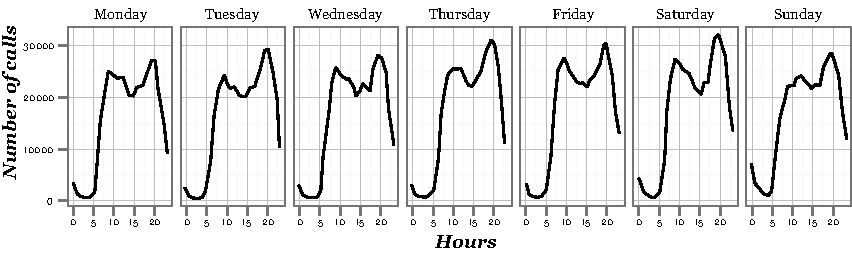
\includegraphics[scale =0.4] {results/images/calls_number.pdf}
	\label{fig:subfig11}
}
\label{fig:fig1}
\end{figure}

As the above picture shows, we can see two peaks $p_1$ from 7 Am to 9 Am and another one $p_2$ from 6 Pm to 8 Pm. As we can see $p_1 > p_2$ in a number of call terms and $p_2$ start to grow at 6 PM and get its maximum value at 8 PM, after this hour, the number of calls dicrease linearly. Another main thing showed by the picture is that exists a central valley between $p_1$ and $p_2$, i.e.:  from 9 Am to 6 Pm, that people stop or relax the number of calls. 
This main component is common to the seven days of the week, therefore, we can assume that people have the same behavior.
\\
\\
Several assumptions could be suggested at this point, for instance, in the $p_1$ range, people start to work or the regular daily activite, in the central valley, some people stop, for example, to eat, and in the next peak $p_2$, people return to regular daily activite and perhaps return to our homes. This last assumption, will be tested with the proposed model and the final GIS visualization and is the central core of our work. The question is figure out the commuting dynamic through the average displacement per person and where are the time ranges that people realize this action.
Datasets has been processed carried out by the mathematical model proposed, therefor, static users has been removed and dinamyc users, better, its tracks has been grouped into a temporal windows and grouped by the day of the week. Seven pictures are shown below in and their respective data tables.


\begin{figure}[ht]
\centering
\subfigure[Total number of calls grouped by Week days]{
	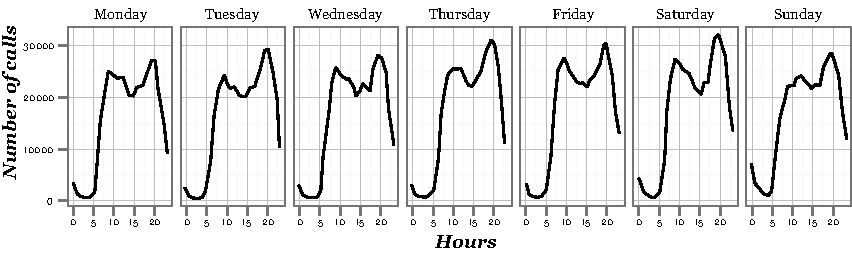
\includegraphics[scale =0.4] {results/images/calls_number.pdf}
	\label{fig:subfig11}
}
\label{fig:fig1}
\end{figure}




